\chapter{Проектируем конкурентное приложение}
\begin{wrapfigure}{r}{0.35\linewidth}
    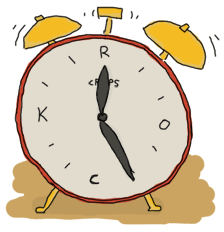
\includegraphics[width=1\linewidth]{clock.png}
\end{wrapfigure}
Это всё прекрасно и хорошо.
Вы усвоили концепции, но, опять же, мы с самого начала книги занимались лишь игрушечными примерами: калькуляторами, деревьями, ездили из Хитроу в Лондон и т.д.
Пора сделать что\--нибудь более интересное с точки зрения обучения.
Мы напишем небольшое приложение на конкурентном Erlang.
Приложение будет линейным и простым, но в то же время полезным и в меру расширяемым.

Я немного неорганизованный человек.
Я запутался в домашних заданиях, благоустройстве квартиры, этой книге, работе, совещаниях, встречах и прочем.
У меня есть дюжина списков с задачами, которые я забываю сделать, или просто не нахожу для них времени.
Надеюсь, вам тоже иногда нужно напоминать о делах (хоть ваш разум  и не блуждает так же часто как мой), потому что мы напишем что\--то вроде приложения для напоминания о событиях, которое уведомляет о необходимости что\--либо сделать и напоминает о встречах.
\section{Разбираем задачу}
Перво\--наперво нужно понять, что мы вообще собираемся сделать.
Вы скажете: <<Напоминалку>>.
<<Ну, конечно>>, \--- скажу я.
Но это ещё не всё.
Как мы собираемся взаимодействовать с программой?
Что она должна для нас делать?
Как представить программу при помощи процессов?
Как узнать, какие нужно отсылать сообщения?

Как говорится: "Ходить по воде и разрабатывать программное обеспечение по техническому заданию одинаково просто, если и то и другое заморожено."
Так что давайте разработаем технические условия и будем их придерживаться.
Наша программа позволит совершать следующие действия:
\begin{itemize}
\item Добавлять событие.
У событий может быть крайний срок исполнения (момент времени, о котором необходимо предупредить), наименование события и его описание.
\item Показывать предупреждение, когда подошло время.
\item Отменять событие по его имени.
\item Не хранить данные на диске.
Для демонстрации архитектурных концепций, которые мы рассмотрим, это совершенно излишне.
Для настоящего приложения это, конечно никуда не годится, но вместо создания этой функциональности, я покажу, куда можно вставить код, если бы вам захотелось её реализовать, и укажу на несколько полезных функций, которые могли бы вам в этом помочь.
\item Так как постоянного хранилища у нас нет, мы должны иметь возможность изменять код во время исполнения.
\item Общение с программой будет осуществляться через командную строку, но мы должны предусмотреть возможность последующего расширения  средств взаимодействия (добавить, скажем, графический интерфейс, доступ через веб\--страницу, через систему обмена мгновенными сообщениями (instant messaging), е\--мейл и прочее).
\end{itemize}

Для нашей программы я избрал такой способ организации:
\begin{figure}[h!]
    \centering
    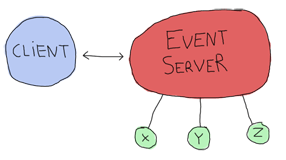
\includegraphics[width=0.4\textwidth]{reminder-structure.png}
\end{figure}

Где клиент, сервер событий и x, y, z представлены в виде процессов.
Вот что каждый из них может делать:
\subsection{Сервер событий}
\begin{itemize}
\item Принимает подписки от клиентов
\item Передаёт уведомления от процессов, генерирующих события, каждому подписчику
\item Принимает сообщения о добавлении событий (и необходимости запуска процессов x, y, z)
\item Может принимать сообщения об отмене события, и последующем убийстве процессов\--генераторов событий
\item Может быть остановлен клиентом
\item Его код может быть перегружен из оболочки.
\end{itemize}
\subsection{Клиент}
\begin{itemize}
\item Подписывается на события у сервера событий и получает уведомления посредством сообщений.
Таким образом, можно легко создать группу клиентов, которые создают подписку на сервере событий.
Каждый клиент потенциально может служить шлюзом к различным точкам взаимодействия, упомянутым выше (графический интерфейс, веб\--страница, программа обмена мгновенными сообщениями, е\--мейл и т.д.)
\item Запрашивает у сервера создание события с необходимыми параметрами
\item Делает запрос к серверу на отмену события
\item Отслеживает сервер (на случай если тот прекратит работу)
\item При необходимости останавливает сервер событий
\end{itemize}
\subsection{x, y и z}
\begin{itemize}
\item С их помощью обозначаются уведомления, готовые к запуску (они реализованы в виде таймеров, связанных с сервером событий)
\item Отсылают сообщение серверу событий по истечении заданного периода
\item Получают сообщение об отмене и умирают
\end{itemize}

Обратите внимание, что все клиенты (IM, почта и т.д., которые в этой книге не реализованы) получают уведомления обо всех событиях, а отмена обычно не входит в список вещей, о которых следует предупреждать клиентов.
Эта программа предназначена для нас с вами, поэтому считается, что её будет запускать только один пользователь.

Вот более сложная схема, с указанием всех возможных сообщений:
\begin{figure}[h!]
    \centering
    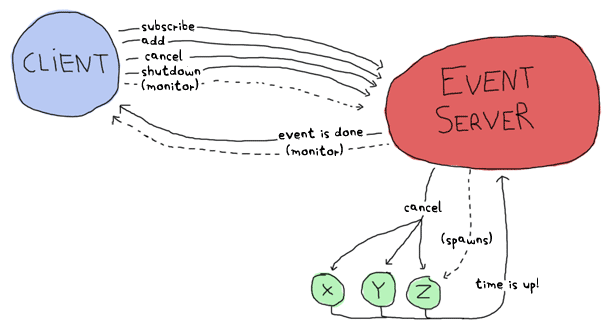
\includegraphics[width=0.7\textwidth]{reminder-bubbles-and-arrows.png}
\end{figure}

Здесь указан каждый процесс, который мы будем использовать.
Стрелки обозначают передаваемые сообщения.
С их помощью мы записали высокоуровневый протокол взаимодействия, ну или хотя бы его основу.

Нужно заметить, что для уведомлений мы используем по процессу на каждое событие.
Это слишком расточительно, и такое решение будет плохо масштабироваться в реальной задаче.
Но для приложения, единственным пользователем которого будете только вы, это вполне уместно.
Можно было бы решить эту проблему иначе, и использовать, к примеру, функцию \href{http://erldocs.com/R15B/stdlib/timer.html\#send_after/2}{timer:send\_after/2-3}, чтобы избежать порождения большого количества процессов.
\clearpage
\section{Определяем протокол}
\label{defining-the-protocol}
Теперь, когда мы знаем что должен передавать каждый компонент и каковы его функции, неплохо было бы составить список всех передаваемых сообщений, и установить их вид.
Начнём с взаимодействия между клиентом и сервером событий:
\begin{figure}[h!]
    \centering
    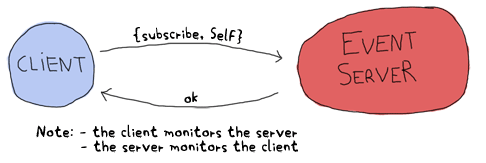
\includegraphics[width=0.6\textwidth]{reminder-subscribe.png}
\end{figure}

Я решил использовать два монитора, так как между клиентом и сервером нет явной зависимости.
Конечно, клиент без сервера не работает, но сервер без клиента существовать сможет.
Здесь можно было бы использовать связь (link), но мы хотим, чтобы функциональность нашей системы могла расширяться за счёт различных клиентов, поэтому мы не можем просто предположить, что после остановки сервера любой клиент тоже захочет аварийно завершиться.
Мы также не можем рассчитывать на то, что клиент можно превратить в системный процесс, и он начнёт улавливать завершения (exits) в случае смерти сервера.
Перейдём к следующему набору сообщений:
\begin{figure}[h!]
    \centering
    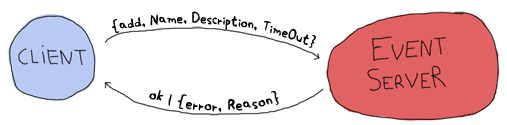
\includegraphics[width=0.6\textwidth]{reminder-add.png}
\end{figure}

Здесь мы добавляем на сервере событий ещё одно событие.
Клиенту высылается подтверждение в виде атома \ops{ok}, за исключением случаев, когда что\--то пошло не так (может, TimeOut был передан в неверном формате.)
Обратная операция удаления событий может быть совершена следующим образом:
\begin{figure}[h!]
    \centering
    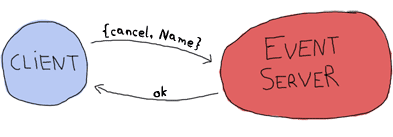
\includegraphics[width=0.6\textwidth]{reminder-remove.png}
\end{figure}

Позже сервер событий может отослать уведомление о том, что событие наступило:
\begin{figure}[h!]
    \centering
    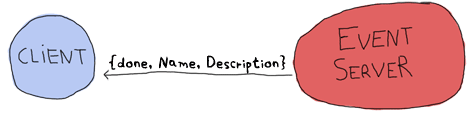
\includegraphics[width=0.6\textwidth]{reminder-cs-done.png}
\end{figure}

Нам осталось определить пару особых случаев: когда необходимо остановить сервер, и когда сервер аварийно завершается:
\begin{figure}[h!]
    \centering
    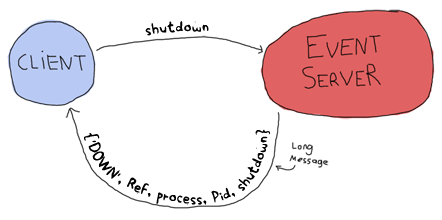
\includegraphics[width=0.6\textwidth]{reminder-shutdown.png}
\end{figure}

Прямое подтверждение об остановке  сервера не отсылается, так как о случившемся нас предупредит монитор.
Вот, в общем\--то и всё, что будет происходить между клиентом и сервером событий.
Перейдём к сообщениям, передаваемым между сервером событий и самими процессами событий.

Перед тем как мы начнём, я бы хотел заметить, что неплохо было бы установить связи между сервером событий и событиями.
Сделать это нужно по той причине, что если сервер умирает, нам нужно чтобы все события умерли вместе с ним \--- без сервера в них нет никакого смысла.

Хорошо, вернёмся к событиям.
Когда сервер событий их создаёт, он присваивает каждому особый идентификатор (имя события).
Как только приходит время какого\--нибудь события, сервер должен отослать уведомляющее сообщение:
\begin{figure}[h!]
    \centering
    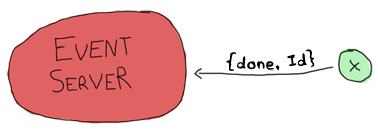
\includegraphics[width=0.6\textwidth]{reminder-es-done.png}
\end{figure}

\clearpage
Событие, в свою очередь, должно ожидать от сервера событий сигналы об отмене:
\begin{figure}[h!]
    \centering
    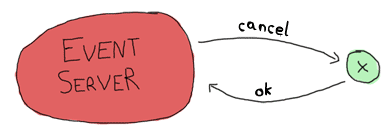
\includegraphics[width=0.6\textwidth]{reminder-cancel.png}
\end{figure}

Мы почти закончили.
Нам потребуется ещё одно последнее сообщение, которое позволит обновлять код сервера:
\begin{figure}[h!]
    \centering
    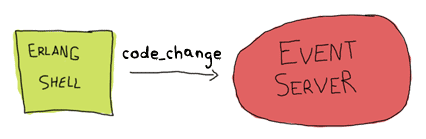
\includegraphics[width=0.6\textwidth]{reminder-code-change.png}
\end{figure}

Отвечать на это сообщение нет необходимости.
Когда мы реализуем эту часть нашей программы, вы поймёте почему мы можем так делать.

Теперь у нас есть и протокол общения, и приблизительная структура иерархии процессов.
Мы можем наконец\--то начать воплощение нашего проекта в жизнь.
